\section*{Statement on the Use of Large Language Models}

In the interest of transparency and in compliance with the ICLR 2026 guidelines, we report that a large language model (LLM) was used to assist in the refinement of this paper's text.

\paragraph{Scope of Use.} 
The model's role was strictly limited to that of a writing assistant. Its contributions include:
\begin{itemize}
    \item Correcting grammatical errors, spelling, and punctuation.
    \item Improving sentence structure and flow for enhanced clarity.
    \item Refining word choices for greater precision and conciseness.
\end{itemize}

\begin{figure*}[htb!]
\centerline{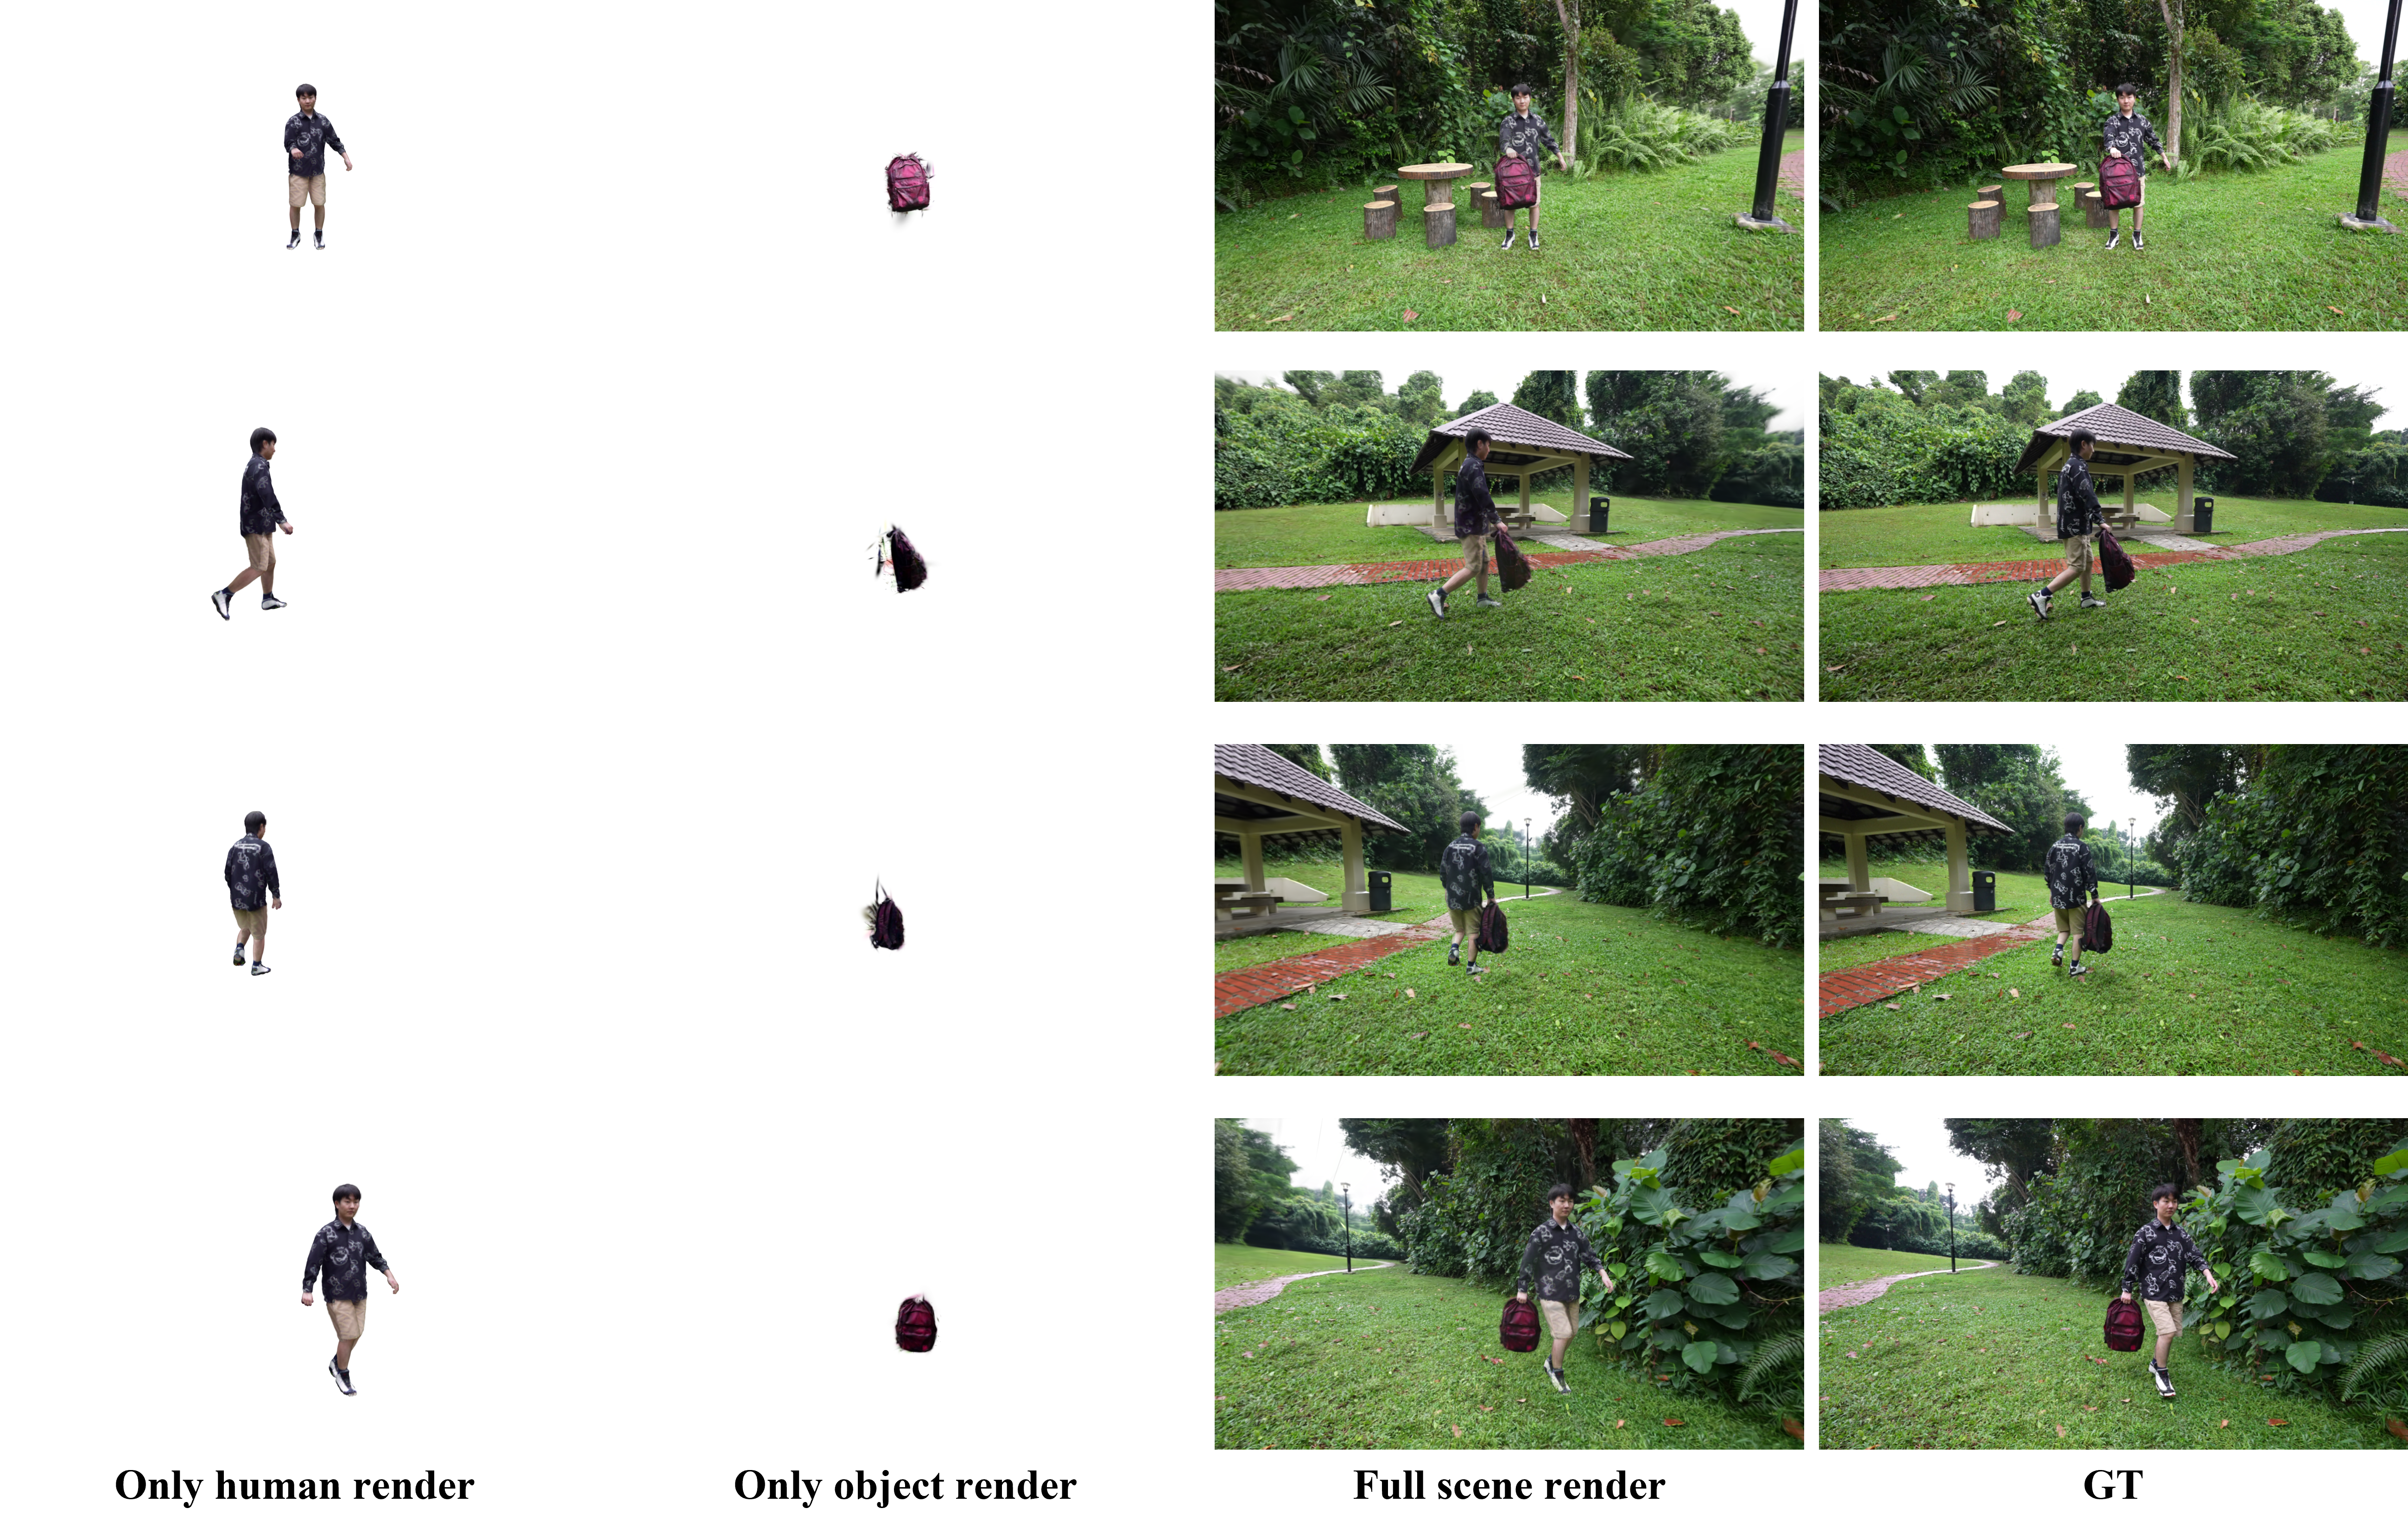
\includegraphics[width=\textwidth]{iclr2026/images/appendix/Appendix_1.png}}
    \vspace{-2mm}
    \caption{\textbf{Decomposed scene reconstruction.}
    Visualization of individual scene components demonstrating geometric integrity in occluded regions. From left to right: human-only rendering, object-only rendering, full scene rendering, and ground truth. Each row shows a different frame from the sequence, highlighting that both human and object maintain coherent geometry even during close contact and occlusion.}
    \label{fig:decomposed_render}
\end{figure*}

\subsection{Decomposed Visualization}
\textcolor{blue}{
\textbf{Component-level Reconstruction Quality.} 
To address concerns about reconstruction quality in occluded regions, we provide decomposed visualizations that isolate individual scene components. As shown in Figure~\ref{fig:decomposed_render}, we render the human and object separately to demonstrate that each component maintains geometric integrity even in regions with heavy occlusion or contact.}

\textcolor{blue}{
\textbf{Human-only Rendering (Column 1):} The isolated human reconstruction shows coherent body geometry throughout the sequence, including regions that were occluded by the object (backpack) in the original footage. This demonstrates that our hexplane-based human deformation successfully captures the complete body structure without artifacts from the interacting object.}

\textcolor{blue}{
\textbf{Object-only Rendering (Column 2):} The object is reconstructed as a distinct, stable entity with well-defined geometry. Unlike single-field approaches that often produce fused or melted geometry at contact points, our CHS-based object deformation maintains clear boundaries and structural consistency throughout the interaction.}

\textcolor{blue}{
\textbf{Full Scene Rendering (Column 3):} The combined rendering seamlessly integrates both components and closely matches the ground truth, confirming that our explicit modeling of human-object interactions through the HOI module enables accurate disentanglement while preserving realistic appearance.}

\textcolor{blue}{
These results validate that HOIGS does not simply overfit the combined RGB appearance but genuinely learns separate geometric representations for humans and objects. The clean separation at contact boundaries and the preservation of geometry in occluded regions demonstrate the effectiveness of our approach in handling complex interaction scenarios.
}
\subsection{Quantitative Evaluation of Human Pose Accuracy}

\begin{table*}[t]
\centering
\tiny
\setlength\tabcolsep{1.0pt}
\def\arraystretch{1.4} % Increased slightly for better separation of slashed values
\resizebox{\textwidth}{!}{%
\begin{tabular}{C{2.5cm}|C{3.2cm}C{3.2cm}C{3.2cm}C{3.2cm}}
\specialrule{.1em}{.05em}{.05em}

% -------- Part 1: First 4 Classes --------
\textbf{Model} &
\textbf{Backpack1} &
\textbf{Plasticcontainer1} &
\textbf{Plasticcontainer2} &
\textbf{Suitcase1} \\ \hline

ExAvatar & 
0.4196 / 0.4628 / 0.3687 & 
0.3875 / 0.4282 / 0.3563 & 
0.3094 / 0.3145 / 0.2897 & 
0.2654 / 0.2957 / 0.2505 \\

HOIGS (Ours) & 
0.4177 / 0.4539 / 0.3656 & 
0.2964 / 0.3344 / 0.2863 & 
0.2973 / 0.3120 / 0.2837 & 
0.2438 / 0.2649 / 0.2352 \\

\specialrule{.1em}{.05em}{.05em}

% -------- Part 2: Next 4 Classes --------
\textbf{Model} &
\textbf{Backpack2} &
\textbf{Plasticcontainer3} &
\textbf{Backpack3} &
\textbf{Trashbin} \\ \hline

ExAvatar & 
0.2690 / 0.3135 / 0.2488 & 
0.3293 / 0.3298 / 0.2970 & 
0.2177 / 0.2494 / 0.2092 & 
0.2294 / 0.2597 / 0.2156 \\

HOIGS (Ours) & 
0.2629 / 0.3068 / 0.2438 & 
0.3270 / 0.3265 / 0.2948 & 
0.2110 / 0.2380 / 0.2020 & 
0.2263 / 0.2550 / 0.2126 \\

\specialrule{.1em}{.05em}{.05em}

\end{tabular}%
}
\caption{
Unified quantitative evaluation on the BEHAVE dataset. The values in each cell correspond to \textbf{PA-MPJPE / PA-MPJPE (Hand/Forearm) / PA-PVE}. HOIGS consistently outperforms the baseline across these metrics, particularly in interaction-critical regions.
}
\label{tab:unified_comparison}
\end{table*}


\textcolor{blue}{
\textbf{Geometric Fidelity Analysis}. 
We acknowledge that rendering metrics alone are insufficient to fully validate the geometric fidelity of complex human–object interactions. To address this, we conducted additional evaluations on human pose accuracy using the BEHAVE dataset. We compare our method against ExAvatar using PA-MPJPE (Procrustes Aligned Mean Per Joint Position Error) and PA-PVE (Procrustes-Aligned Per Vertex Error).
}

\begin{figure*}[htb!]
\centerline{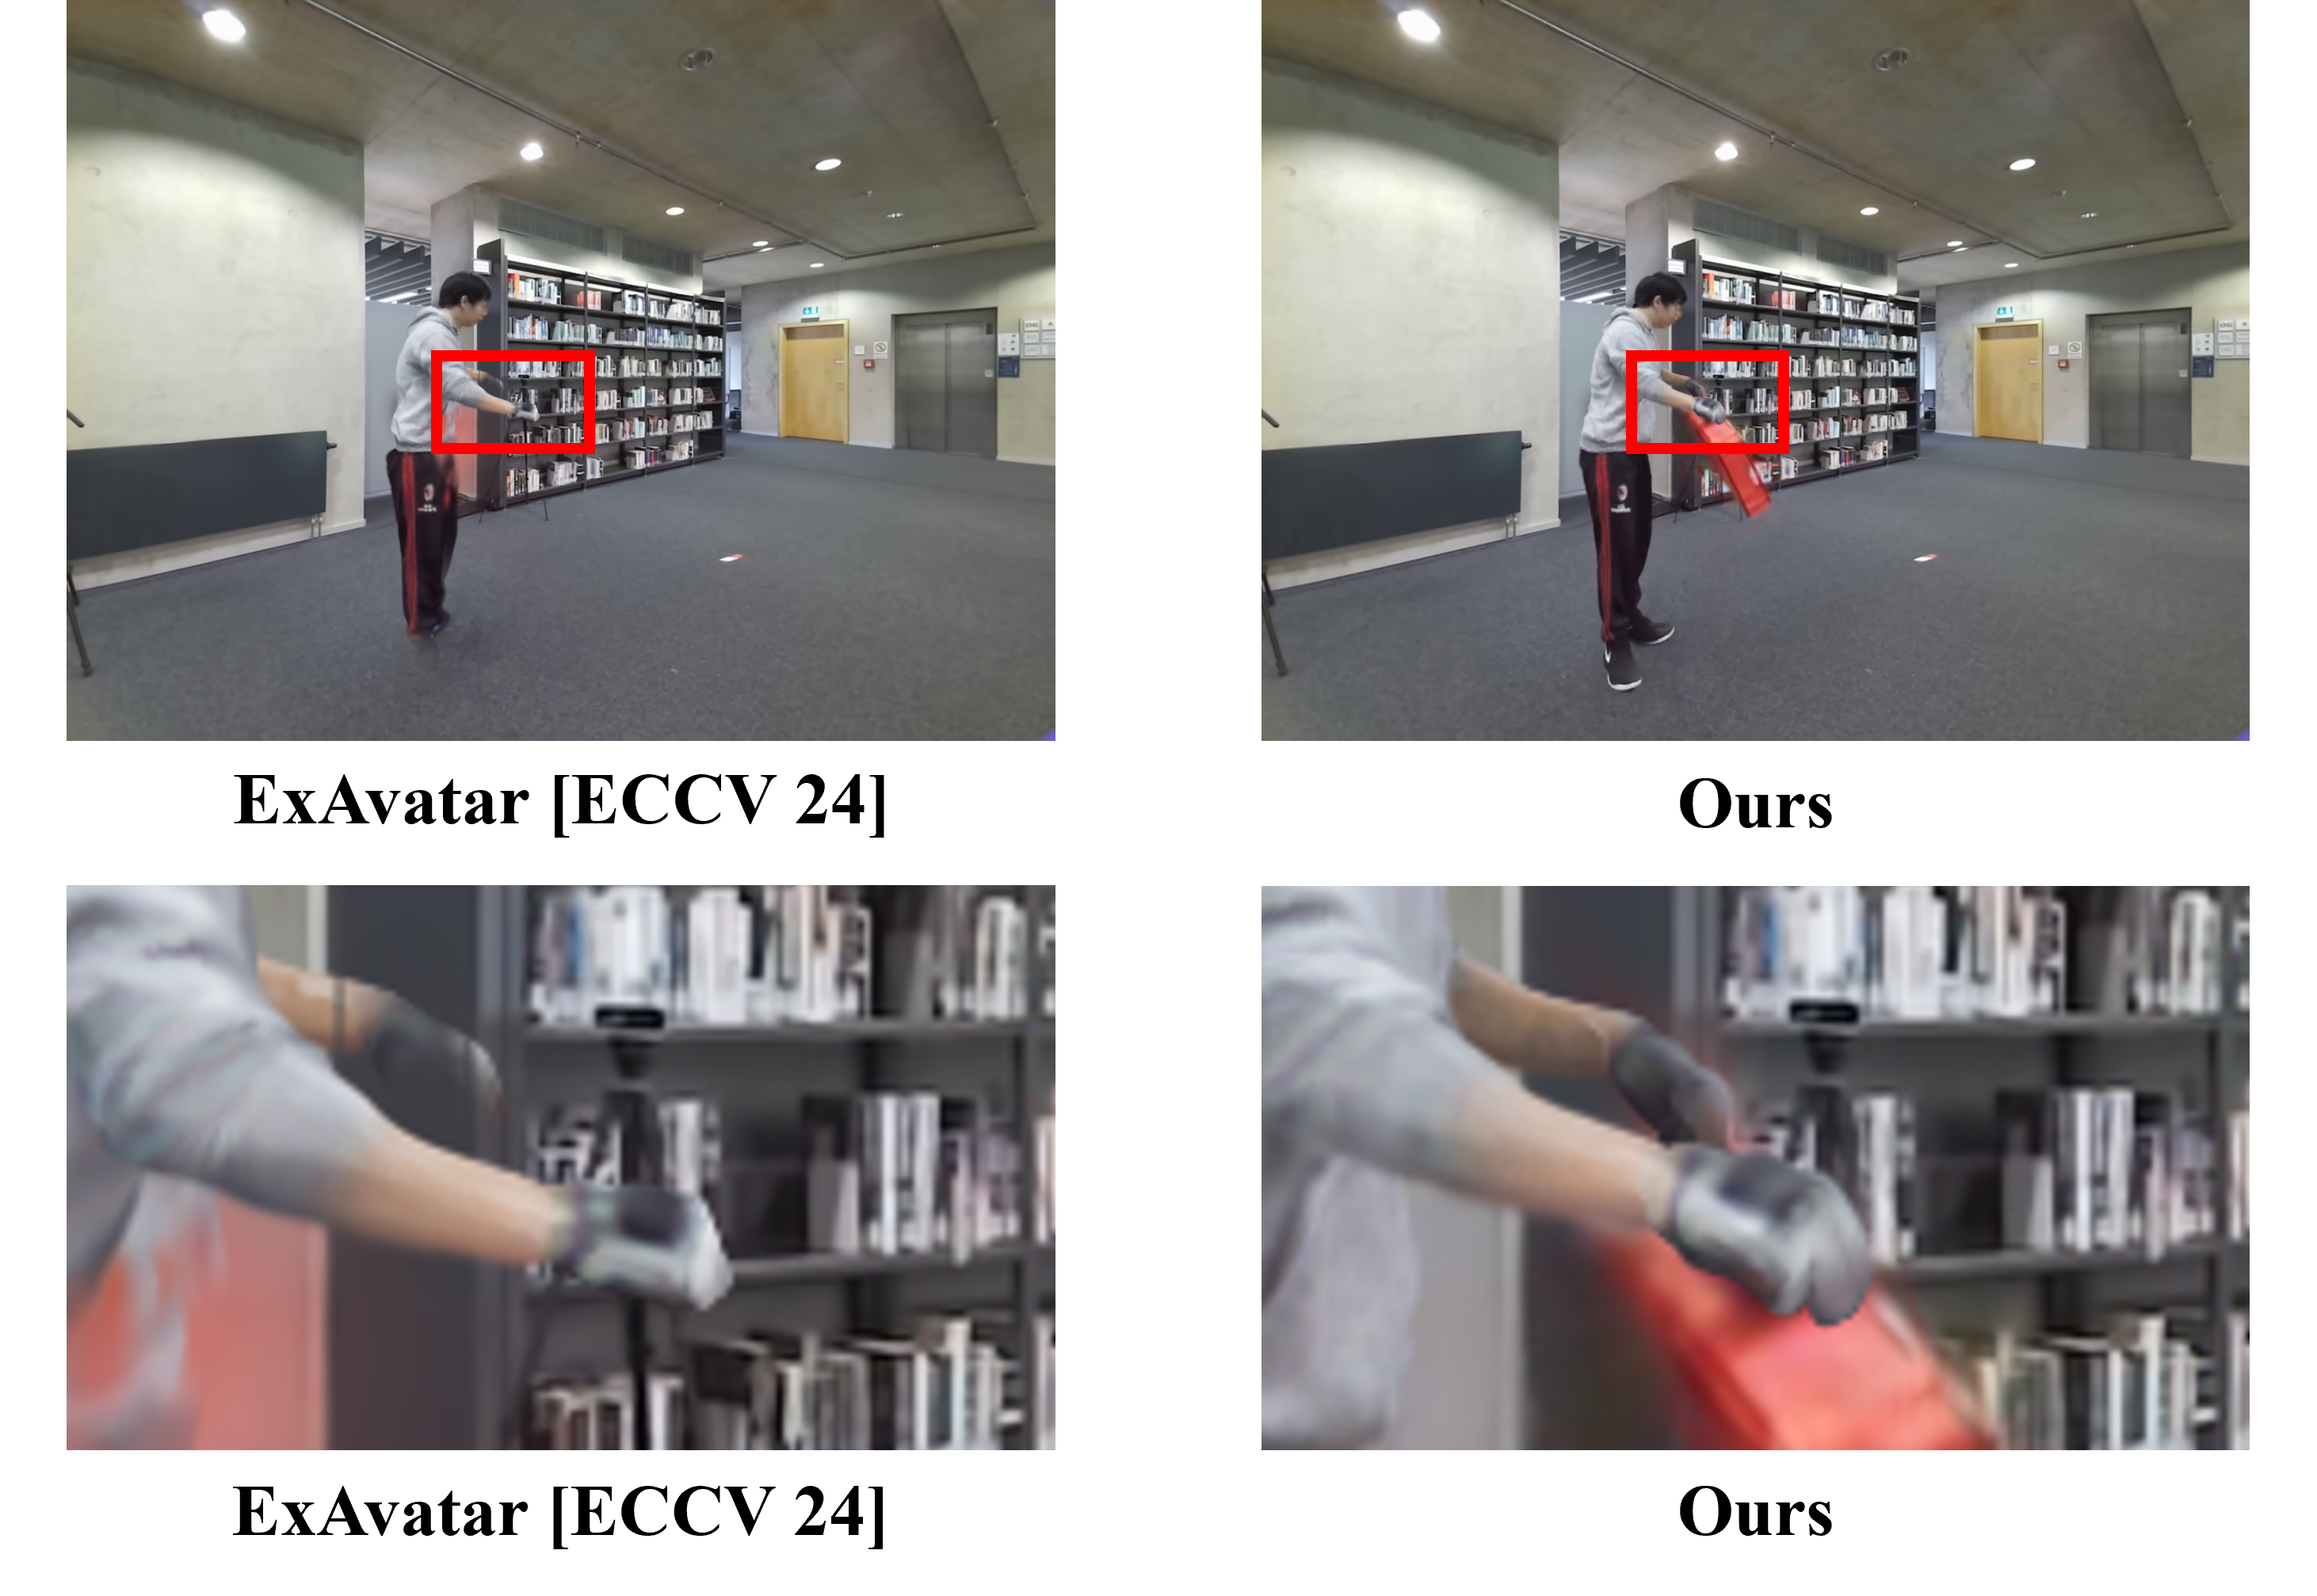
\includegraphics[width=\textwidth]{iclr2026/images/appendix/behave_refine.png}}
    \vspace{-2mm}
    \caption{\textbf{Qualitative comparison of human pose refinement on the BEHAVE dataset.}
    Visual comparison between ExAvatar and our method (HOIGS). The red boxes highlight the interaction regions (hands and objects). Our HOI module explicitly refines the hand and forearm poses by leveraging object motion features, leading to accurate contact modeling, whereas ExAvatar exhibits misalignment in these interaction-rich regions.}
    \label{appendix_behave_refine}
\end{figure*}


\textcolor{blue}{
\textbf{Effect of the HOI Module on Pose Refinement}.
Our method explicitly models the mutual dependency between the human and the object. The HOI module leverages a cross-attention mechanism to use object motion features as contextual cues to refine human features. Specifically, as described in Eq. 14 of the main paper, the module predicts refinement offsets $\Delta$SMPL-X for the body and hands. This capability allows the network to correct the human pose—even under partial occlusion—by inferring the likely body configuration from the object's trajectory.
}


\textcolor{blue}{
\textbf{Quantitative Results}.
Table \ref{tab:unified_comparison} summarizes the evaluation on the BEHAVE dataset. We report the average PA-MPJPE and PA-PVE across all test frames. Additionally, we provide a specific analysis for Hand and Forearm joints, which are the most critical regions for interaction tasks.
}
\textcolor{blue}{
As shown in Table \ref{tab:unified_comparison}, HOIGS consistently outperforms the baseline. Notably, we observe a larger performance gain in the \textbf{PA-MPJPE (Hand/Forearm joints)}. This indicates that our HOI module effectively refines the poses of interaction-related body parts, resulting in physically more accurate reconstructions compared to ExAvatar, which lacks mutual feedback between the human and the object. Please refer to the per-sequence detailed tables at the bottom of the appendix.}

\subsection{Sensitivity Analysis on External Modules}

\begin{table*}[t]
\centering
\small
\setlength\tabcolsep{1.0pt}
\resizebox{\textwidth}{!}{%
\begin{tabular}{C{4.3cm}|C{1.1cm}C{1.1cm}|C{1.1cm}C{1.1cm}|C{1.1cm}C{1.1cm}|C{1.1cm}C{1.1cm}|C{1.1cm}C{1.1cm}|C{1.1cm}C{1.1cm}|C{1.1cm}C{1.1cm}}
\specialrule{.1em}{.05em}{.05em}
\multirow{2}{*}{Method Combinations} &
\multicolumn{2}{c|}{\textbf{Backpack}} &
\multicolumn{2}{c|}{\textbf{Tennis}} &
\multicolumn{2}{c|}{\textbf{Suitcase}} &
\multicolumn{2}{c|}{\textbf{Playground}} &
\multicolumn{2}{c|}{\textbf{Dance}} &
\multicolumn{2}{c|}{\textbf{Lounge}} &
\multicolumn{2}{c}{\textbf{Average}} \\
& PSNR$\uparrow$ & LPIPS$\downarrow$
& PSNR$\uparrow$ & LPIPS$\downarrow$
& PSNR$\uparrow$ & LPIPS$\downarrow$
& PSNR$\uparrow$ & LPIPS$\downarrow$
& PSNR$\uparrow$ & LPIPS$\downarrow$
& PSNR$\uparrow$ & LPIPS$\downarrow$ 
& PSNR$\uparrow$ & LPIPS$\downarrow$ \\ \hline

Samurai + MetricV2
& 25.78 & 0.082 
& 27.12 & 0.108 
& 22.09 & 0.246 
& 25.23 & 0.103 
& 24.17 & 0.098 
& 30.97 & 0.048 
& 25.89 & 0.114 \\

Samurai + Video Depth Anything
& 25.85 & 0.080 
& 27.18 & 0.106 
& 22.15 & 0.241 
& 25.28 & 0.102 
& 24.22 & 0.096 
& 31.05 & 0.046 
& 25.96 & 0.112 \\

Samurai + DepthCrafter
& 25.72 & 0.088 
& 27.08 & 0.108 
& 22.06 & 0.249 
& 25.20 & 0.109 
& 24.08 & 0.099 
& 30.93 & 0.048 
& 25.85 & 0.117 \\

TrackAnything + MetricV2
& 25.72 & 0.086 
& 27.05 & 0.109 
& 22.03 & 0.246 
& 25.18 & 0.106 
& 24.15 & 0.100 
& 30.93 & 0.052 
& 25.84 & 0.116 \\

SAMv2 + Video Depth Anything
& 26.01 & 0.076 
& 27.38 & 0.103 
& 22.33 & 0.241 
& 25.47 & 0.100 
& 24.42 & 0.095 
& 31.20 & 0.041 
& 26.14 & 0.109 \\

MaskRCNN + MetricV2
& 25.33 & 0.099 
& 26.67 & 0.125 
& 21.66 & 0.257 
& 24.78 & 0.117 
& 23.69 & 0.110 
& 30.52 & 0.065 
& 25.44 & 0.129 \\

\specialrule{.1em}{.05em}{.05em}
\end{tabular}%
}
\caption{
Sensitivity analysis of HOIGS on the HOSNeRF dataset using different combinations of segmentation and depth estimation priors. The results demonstrate the robustness of our method, with consistent performance across various modern priors and strong performance even with older baselines (MaskRCNN).
}
\label{tab:sensitivity_analysis}
\end{table*}


\textcolor{blue}{
\textbf{Robustness to External Priors.}~
To address concerns regarding the reliance on external modules, we conducted a sensitivity analysis on the HOSNeRF dataset by evaluating our framework with various combinations of segmentation (e.g., Samurai~\cite{yang2024samurai}, SAMv2~\cite{ravi2024sam2}, MaskRCNN~\cite{massa2018mrcnn}, TrackAnything~\cite{yang2023track}) and depth estimation (e.g., Video Depth Anything~\cite{video_depth_anything}, MetricV2~\cite{hu2024metric3dv2}, DepthCrafter~\cite{hu2025-DepthCrafter}) models.~
As shown in Table~\ref{tab:sensitivity_analysis}, HOIGS maintains highly consistent performance (Avg PSNR 25.8--26.1) across different modern priors, demonstrating that our method is robust to variations in preprocessing quality.~
Notably, even when employing the standard, older baseline of MaskRCNN combined with MetricV2, our model achieves an average PSNR of 25.44.~
This performance remains significantly higher than the state-of-the-art human-centric baseline, ExAvatar (Avg PSNR 24.35), and the 4DGS baseline, Ex4DGS (Avg PSNR 17.97).
}


% \textcolor{blue}{
% \textbf{Robustness to External Priors.} 
% To address concerns regarding the reliance on external modules, we conducted a sensitivity analysis on the HOSNeRF dataset by evaluating our framework with various combinations of segmentation (e.g., Samurai, SAMv2, MaskRCNN, TrackAnything) and depth estimation (e.g., Video Depth Anything, MetricV2, DepthCrafter) models. 
% As shown in Table~\ref{tab:sensitivity_analysis}, HOIGS maintains highly consistent performance (Avg PSNR 25.8--26.1) across different modern priors, demonstrating that our method is robust to variations in preprocessing quality. 
% Notably, even when employing the standard, older baseline of MaskRCNN combined with MetricV2, our model achieves an average PSNR of 25.44. 
% This performance remains significantly higher than the state-of-the-art human-centric baseline, ExAvatar (Avg PSNR 24.35), and the 4DGS baseline, Ex4DGS (Avg PSNR 17.97).
% }

 
\subsection{Computational Complexity and Runtime Analysis}
\textcolor{blue}{
\textbf{Runtime Performance}.
We evaluate the computational efficiency of our method on the HOSNeRF dataset using a single NVIDIA H100 GPU. As shown in Table~\ref{tab:runtime_comparison}, our method achieves an inference speed of \textbf{44.27 FPS}. While this is slightly lower than 4DGS~\cite{wu20244d} (61.04 FPS), it remains comparable to Ex4DGS~\cite{lee2024fully} (46.38 FPS) and outperforms D3DGS~\cite{yang2024deformable} (37.79 FPS). This result confirms that the inclusion of the HOI attention mechanism does not create a significant bottleneck, allowing our method to comfortably support real-time applications.
}
\begin{table}[t] % Changed [h] to [t] or [ht] for better float placement
\centering
\small
\setlength\tabcolsep{8.0pt}
% Using resizebox to match your style
\resizebox{0.7\textwidth}{!}{%
\begin{tabular}{l|c|c}
\specialrule{.1em}{.05em}{.05em}
\textbf{Methods} & \textbf{Training Time} & \textbf{Inference Speed (FPS)} \\ \hline
4DGS~\cite{wu20244d} & 40 min & 61.04 \\
Ex4DGS~\cite{lee2024fully} & 2 hr 30 min & 46.38 \\
D3DGS~\cite{yang2024deformable} & 3 hr & 37.79 \\
E-D3DGS~\cite{bae2024per} & 2 hr & 54.71 \\ \hline
\textbf{HOIGS (Ours)} & 5 hr & 44.27 \\
\specialrule{.1em}{.05em}{.05em}
\end{tabular}%
}
\caption{
Runtime performance comparison on the HOSNeRF dataset. We report the approximate training time per scene and the inference speed in Frames Per Second (FPS). Our method maintains real-time performance ($>$30 FPS) despite the added complexity of interaction modeling.
}
\label{tab:runtime_comparison}
\end{table}

\textcolor{blue}{
\textbf{Complexity Analysis}.
The efficiency of our HOI module stems from the token-based architectural design. The cross-attention is computed between $M$ human part tokens (where $M=16$ is fixed) and $N$ object Gaussian tokens. Unlike standard self-attention which scales quadratically ($O(N^2)$), our cross-attention scales linearly ($O(M \cdot N)$) with respect to the number of object Gaussians. Furthermore, we utilize compact 32-dimensional embeddings for object motion features, which minimizes the memory footprint and matrix multiplication overhead during the forward pass.
}

\textcolor{blue}{
\textbf{Training Cost Justification}.
We acknowledge that our training time ($\sim$5 hours) is longer than the baselines. This is a deliberate trade-off to prioritize physical plausibility and interaction accuracy. Explicitly modeling mutual dependencies and backpropagating gradients through the attention mechanism requires more iterations. However, this cost is strictly confined to the offline training phase, ensuring that the final online user experience remains real-time.
}

\begin{table*}[t]
\centering
\small
\setlength\tabcolsep{1.0pt}
\resizebox{\textwidth}{!}{%
\begin{tabular}{l|C{1.1cm}C{1.1cm}|C{1.1cm}C{1.1cm}|C{1.1cm}C{1.1cm}|C{1.1cm}C{1.1cm}|C{1.1cm}C{1.1cm}|C{1.1cm}C{1.1cm}|C{1.1cm}C{1.1cm}}
\specialrule{.1em}{.05em}{.05em}
\multirow{2}{*}{Methods} &
\multicolumn{2}{c|}{\textbf{Backpack}} &
\multicolumn{2}{c|}{\textbf{Tennis}} &
\multicolumn{2}{c|}{\textbf{Suitcase}} &
\multicolumn{2}{c|}{\textbf{Playground}} &
\multicolumn{2}{c|}{\textbf{Dance}} &
\multicolumn{2}{c|}{\textbf{Lounge}} &
\multicolumn{2}{c}{\textbf{Average}} \\
& PSNR$\uparrow$ & LPIPS$\downarrow$
& PSNR$\uparrow$ & LPIPS$\downarrow$
& PSNR$\uparrow$ & LPIPS$\downarrow$
& PSNR$\uparrow$ & LPIPS$\downarrow$
& PSNR$\uparrow$ & LPIPS$\downarrow$
& PSNR$\uparrow$ & LPIPS$\downarrow$
& PSNR$\uparrow$ & LPIPS$\downarrow$ \\ \hline

MASt3R Prior
& 23.51 & 0.135
& 25.25 & 0.121
& 22.40 & 0.197
& 24.65 & 0.074
& 23.63 & 0.115
& 28.99 & 0.057
& 24.59 & 0.128 \\

Depth Recon Prior
& 21.63 & 0.142
& 25.65 & 0.122
& 22.13 & 0.230
& 25.24 & 0.103
& 24.08 & 0.123
& 28.95 & 0.095
& 25.36 & 0.136 \\

\hline
\textbf{Diffusion Prior (Ours)}
& 23.70 & 0.082
& 27.13 & 0.112
& 22.96 & 0.235
& 25.63 & 0.123
& 24.17 & 0.093
& 29.97 & 0.043
& 25.89 & 0.114 \\

\specialrule{.1em}{.05em}{.05em}
\end{tabular}%
}
\caption{
Quantitative ablation study on Object Priors using the HOSNeRF dataset. We evaluate the effectiveness of our Diffusion Prior against MASt3R and Depth Reconstruction priors.
}
\label{tab:prior_ablation}
\end{table*}

\subsection{Additional Ablation Studies}

\textcolor{blue}{
\textbf{Impact of Object Diffusion Prior.} 
To validate the effectiveness of our design choice, we investigate the impact of different geometric priors on the final reconstruction quality. We compare our proposed method, which utilizes a generative Diffusion Prior, against two alternative initialization strategies:\\
(1) MASt3R Prior: Initialization using MASt3R, a state-of-the-art dense matching and reconstruction model. \\
(2) Depth Reconstruction Prior: Initialization using standard monocular metric depth estimation.
}

\textcolor{blue}{
Table \ref{tab:prior_ablation} presents the quantitative comparison on the HOSNeRF dataset. 
Our method equipped with the Diffusion Prior achieves the highest average reconstruction quality (25.89 PSNR), outperforming the MASt3R prior (24.59 PSNR) and the Depth prior (25.36 PSNR).
While discriminative approaches like MASt3R or metric depth estimation rely heavily on visible cues, they often struggle to reconstruct accurate geometry in the presence of heavy occlusions, a common occurrence in human-object interaction scenarios (e.g., hands covering objects).
In contrast, the Diffusion Prior leverages generative knowledge to plausibly complete 3D geometry even in occluded or unseen regions. This holistic geometric initialization provides a more robust starting point for our Cubic Hermite Spline (CHS) deformation, leading to sharper rendering and more stable tracking throughout the dynamic sequence.
}

\subsection{Feature extraction}

\input{images_tex/appendix_object_feature}

\textbf{Object feature}.
%우리는 object feature를 추출하기 위해 key frame의 Gaussian에 대해 velocity vector와 임베딩 파라미터를 활용한다. 각 key frame의 velocity vector는 CHS에 적용되어 baseline deformation과 함께 HOI module의 입력 feature로 공동 최적화된다. 추가적으로 각 key frame의 Gaussian마다 29차원의 learnable parameter를 임베딩하며, 이 임베딩은 velocity vector와 결합되어 feature로 사용된다. CHS를 통해 interpolation된 Gaussian feature는 결합된 feature와 time 정보를 입력으로 받아 얕은 MLP layer를 거쳐 projection되며, 최종적으로 32차원의 feature를 형성한다.
As shown in Fig. \textcolor{blue}{\ref{appendix_objfeature}}(a), we extract object features by leveraging the velocity vectors and embedding parameters of Gaussians at key frames. As shown in Fig. \textcolor{blue}{\ref{appendix_objfeature}}(b), each key frame’s velocity vector is applied to the CHS and jointly optimized with the baseline deformation as input features for the HOI module. In addition, a 29-dimensional learnable parameter is embedded for each key frame Gaussian, which is concatenated with the velocity vector to form the feature representation. The interpolated Gaussian features produced by CHS are then combined with the concatenated feature and time information, and projected through a shallow MLP, resulting in a 32-dimensional feature vector.


\textbf{Human feature}.
Fig. \textcolor{blue}{~\ref{appendix_humanfeature}} illustrates the process of human feature extraction. 
We divide the SMPL-X model into 16 body parts and learn features corresponding to each part. 
Temporal features are sampled from the hexplane at SMPL-X vertices, where each feature at time $t$ is obtained based on the coordinates $(x_t, y_t, z_t)$. 
For each body part, the features of its associated vertices are averaged to form the part-specific representation $F_{\text{human}}$: 
\[
F_{\text{part}} = \frac{1}{N} \sum_{i \in \text{part}} f_i(x_t, y_t, z_t), \tag{10}
\]
where $N$ denotes the number of vertices belonging to the part. 
As a result, 16 part features, including head, torso, arms, and legs, are obtained and used as inputs to the HOI module. 
This design captures temporally varying dynamic representations while preserving semantically meaningful features for individual body parts.



\subsection{HOI module network detail}
As shown in Fig. \textcolor{blue}{\ref{appendix_HOINetwork}}, the proposed HOI module takes the time-varying features of humans and objects as inputs and explicitly models their interactions.
Let the human feature be denoted as $F_{\text{Human}} \in \mathbb{R}^{N_h \times d}$ and the object feature as $F_{\text{Object}} \in \mathbb{R}^{N_o \times d}$, 
where $N_h$ and $N_o$ are the numbers of feature tokens for human and object respectively, and $d$ is the feature dimension. 

To capture interdependencies between the two modalities, we apply a \textit{mutual-attention} mechanism. 
Specifically, queries ($Q$), keys ($K$), and values ($V$) are obtained via learnable linear projections:
\begin{equation}
Q_h = F_{\text{Human}}W_h^Q,\;\; K_o = F_{\text{Object}}W_o^K,\;\; V_o = F_{\text{Object}}W_o^V, \tag{11}
\end{equation}
\begin{equation}
Q_o = F_{\text{Object}}W_o^Q,\;\; K_h = F_{\text{Human}}W_h^K,\;\; V_h = F_{\text{Human}}W_h^V, \tag{12}
\end{equation}
where $W_h^Q, W_h^K, W_h^V, W_o^Q, W_o^K, W_o^V \in \mathbb{R}^{d \times d}$ are learnable projection matrices. 

Cross-attention is then computed in both directions: from human to object and from object to human. 
To enforce spatial priors, a distance mask $B \in \mathbb{R}^{N_h \times N_o}$ is added to the attention logits, where $B_{ij}$ encodes the relative distance between the $i$-th human token and the $j$-th object token. 
The resulting attention maps are defined as:
\begin{equation}
A_{h \leftarrow o} = \text{softmax}\!\left(\tfrac{Q_hK_o^\top}{\sqrt{d}} + B\right),\quad
A_{o \leftarrow h} = \text{softmax}\!\left(\tfrac{Q_oK_h^\top}{\sqrt{d}} + B^\top\right). \tag{13}
\end{equation}

Using these attention weights, the updated features are obtained as:
\begin{equation}
F'_{\text{Human}} = A_{h \leftarrow o} V_h,\quad
F'_{\text{Object}} = A_{o \leftarrow h} V_o. \tag{14}
\end{equation}

The updated human feature $F'_{\text{Human}}$ is then fed into a small MLP head to regress the refinement terms of SMPL-X parameters: 
\[
\Delta \text{SMPL-X} = \{\Delta \theta_{\text{body}},\; \Delta \theta_{\text{hand}}\;\}, \tag{15}
\]
where $\Delta \theta_{\text{body}}$ and $\Delta \theta_{\text{hand}}$ denote pose corrections for body and hands.
Similarly, the updated object feature $F'_{\text{Object}}$ is used to regress Gaussian-based object motion corrections:
\[
\Delta G_{\text{object}} \in \mathbb{R}^{N_o \times 3}, \tag{16}
\]
which represent displacement vectors applied to object Gaussians. 

In this way, the HOI module augments the baseline deformations (hexplane+LBS for humans and CHS for objects) with interaction-aware refinements, enabling accurate reconstruction of complex human--object interaction scenes.

\begin{figure*}[t!]
\centerline{\includegraphics[width=\textwidth]{images/appendix/human_feature.jpg}}
    \vspace{-2mm}
    \caption{\textbf{Human feature extraction.}
    }
    \label{appendix_humanfeature}
    \vspace{-5mm}
\end{figure*}

\subsection{Objective Function Details}
The overall loss function of our model is defined as follows:

\begin{equation}
L = \gamma L_{\text{object motion}} + \beta L_{\text{human}} + \sigma L_{\text{scene}} + L_{\text{depth}}, \tag{17}
\end{equation}

where $L_{\text{object motion}}$, $L_{\text{human}}$, and $L_{\text{scene}}$ correspond to losses for object motion, human modeling, and scene context, respectively. The weights $\gamma$, $\beta$, and $\sigma$ control the relative importance of each loss term and are specifically set to 1.0, 0.5, and 0.25, respectively. In our approach, these three terms are optimized simultaneously to consistently model the interactions between humans and objects.

\textbf{Human Loss details} \\
The $L_{\text{human}}$ term consists of losses related to human representation using the SMPL-X (\textcolor{blue}{\cite{pavlakos2019expressive}}) model. Specifically, it includes the reprojection error between the 3D human joint positions and detected 2D keypoints in images, a mesh-based face loss enhancing the consistency of facial geometry and texture, and a Laplacian regularization term. Additionally, there is an L1 loss ($L_{\text{smplx}}$) between the optimized SMPL-X parameters and the frame-wise initial SMPL-X parameters obtained by a regressor. These loss terms are directly adopted from previous methods such as ExAvatar (\textcolor{blue}{\cite{moon2024expressive}}), without modifications. For example, the face loss optimizes the consistency between rendered facial images and actual facial images, ensuring geometry-texture coherence. Laplacian regularization is applied to enhance the stability of human body shape. Further details can be found in the referenced research.

Formally, the human loss is given by:

\begin{equation}
L_{\text{human}} = L_{\text{kpt}} + L_{\text{face}} + L_{\text{reg}} + 0.1 \times L_{\text{smplx}}, \tag{18}
\end{equation}


\begin{figure*}[t!]
\centerline{\includegraphics[width=0.6\textwidth]{images/appendix/HOINetwork.jpg}}
    \vspace{-2mm}
    \caption{\textbf{Detailed HOI network.}
    The proposed architecture for estimating human-object interactions, leveraging features from human body parts and object Gaussian representations. The model takes as input human part features and per-Gaussian object features, processes them through bidirectional attention mechanisms to incorporate mutual contextual information, and outputs predictions for SMPL-X parameters per body part along with offset adjustments for object Gaussian centers.}
    \label{appendix_HOINetwork}
    \vspace{-5mm}
\end{figure*}
\textbf{Scene Loss details}\\
The $L_{\text{scene}}$ term is a photometric loss focusing on the background regions of the entire scene, following the image similarity-based loss used in existing 3D Gaussian Splatting (\textcolor{blue}{\cite{kerbl20233d}}) (3DGS) methods. Specifically, a pre-trained human/object segmentation model is employed to mask out human and object regions in the images, optimizing the background Gaussians for the remaining pixels only. This involves minimizing the difference between the rendered result and the background pixels excluding the segmented human and object areas. Occlusions frequently occur during interactions between human hands and objects, causing inconsistencies in masks. By optimizing humans, objects, and backgrounds simultaneously, our method effectively mitigates these boundary inconsistencies.

The scene loss is explicitly defined as:

\begin{equation}
L_{\text{scene}} = 0.8 \times L_1(I_{\text{gt}}, I_{\text{render}}) 
+ 0.2 \times L_{\text{D-SSIM}}(I_{\text{gt}}, I_{\text{render}}), \tag{19}
\end{equation}

\textbf{Object Loss details} \\
The $L_{\text{object}}$ term is a photometric loss that focuses exclusively on the object regions within the scene. We render only the segmented object areas and compute the loss solely on these regions. A pre-trained object segmentation model is employed to isolate object masks in the input images. The object loss encourages accurate reconstruction and appearance consistency for moving objects, which often undergo significant deformation and motion. By supervising only the object regions, this loss helps to refine the geometry and texture of the object-specific Gaussians without being influenced by background or human-related elements.

The object loss is defined as:
\begin{equation}
L_{\text{object motion}} = 0.8 \times L_1(I_{\text{gt}}, I_{\text{obj}}) 
+ 0.2 \times L_{\text{D-SSIM}}(I_{\text{gt}}, I_{\text{obj}}). \tag{20}
\end{equation}


 

